\chapter{Results and Discussion}\label{chapter:res}
In this chapter we discuss quantitative and qualitative results from the mobile application and experiments with the baseline DNN; and we make conclusions about the researched approaches. Section \ref{res:performance} covers performance and visual quality of neural rendering in the mobile application. Section \ref{res:training} compares DNN experiments and the impact of the attempted adjustments. Section \ref{res:future} outlooks future research directions to improve the project.

\section{Mobile application results}\label{res:performance}

We compare performance of inferring the baseline DNN at different stages of progress during completion of this thesis project. In the next paragraphs we will analyze Table \ref{tab:mobile-performance}. As was mentioned in Section \ref{methods:dev-setup}, we can measure frame time of the AR application, which includes time of SMPL-X inference, input rasterization, passing it to the DNN, inferring the DNN and rendering the AR content. Alternatively, in our "benchmarking" application mode, we infer the DNN for 5 minutes on the same input data to gather fair statistics on the inference time and maximum increase of the device temperature. However we noticed, that since we initialize SNPE with "Sustained High Performance" profile, the maximum temperature is controlled by the device and it never exceeds $55^\circ$C, thus we do not report it. As per the project task, we consider performance as real-time, if application frame time is below 33 ms, which corresponds to above 30 FPS.

In our initial implementation, when we encountered the limitation of OpenGL for rasterizing images of at most 4 channels, we generated the DNN's input tensors using multiple OpenGL rasterizations of size $H \times W \times 4$. Then the DNN was extended from the PyTorch side to accept these multiple rasterizations, and permute the data in memory to get the necessary $H \times W \times C$ before starting the inference. Although the permutation would take place on the GPU or DSP, the performance was fairly low even for resolution $256 \times 256$ pixels with 8 neural texture channels (row 1 in Table \ref{tab:mobile-performance}). Trying to run this layout for the desired resolution $512 \times 512$ and 16 channels, the performance would drop below 25 FPS (row 2). However, by implementing the quantization and packing of all neural channels with a single OpenGL rasterization and getting the input tensor in the exact memory layout as required, the performance immediately improves for all such resolutions (rows 3,4,5) and becomes real-time on DSP. We could further increase the resolution of rendering, still having real-time performance with $640 \times 640$ pixels (row 6). To test the limits of the hardware, we try $1024 \times 1024$ resolution (row 7), which is obviously beyond real-time, as computations scale quadratically with resolution. On the bright side, the architecture was successfully converted for execution on DSP. In our experience, some neural layers may not work on DSP for high resolutions due to a hardware limit on tensor spatial dimensions or number of channels. Thus practically, such high resolutions are possible on mobile with the architecture we use, yet the performance is the bottleneck. 

Next, following the experiments on the DNN's training procedure, we try to run a modified architecture, with all Batch Normalization (BN) layers replaced with either Instance Normalization or Group Normalization layers. BN layers typically store running exponential average of batch statistics from the training data, thus allowing to use the pre-computed mean and standard deviation for each tensor, and normalize tensors with little to no overhead during inference. Instance and Group Normalization layers, however, by default require computing the statistics on each inference. Thus it is expected of them to have lower performance. As we measure, compared to BN layers, an architecture with Instance Normalization layers is about 30-50\% slower (compare rows 5 and 6; rows 9 and 10), but still borderline real-time. Group Normalization layers are computed very inefficiently (row 13). In fact, documentation of SNPE does not mention support of it, thus it may be computed with hardly any hardware acceleration.

Finally, we examine how different encoder types of the neural renderer affect the performance. While the baseline DNN uses ResNet18 \cite{dnn:resnet16}, it might be expected for light-weight architectures like MobileNet \cite{dnn:mnv2-18,dnn:mnv3-19} or EfficientNet \cite{dnn:efficientnetv1-19} to drastically outperform. However, from out attempts MobileNetV2 is not inferred faster for the same resolutions (rows 9,10,11), even though it has twice as fewer parameters. We speculate, that the depth-wise convolutional layers used in MobileNetV2 have no efficient implementation on the hardware. After replacing BN layers with Instance normalization layers, we observe the similar percent of performance degradation (row 10). MobileNetV3 \cite{dnn:mnv3-19} appears to be a bit faster for resolution $256 \times 256$ (row 14), however we could not convert models with any higher resolution into the SNPE format. We tested out EfficientNet-Lite0  model, and it performs the best for resolution $512 \times 512$, while having a comparable number of parameters to MobileNetV2. However, inference on DSP results in a failed segmentation prediction (see Figure \ref{fig:mobile_tf_effent_fail}). This artifact does not appear with GPU execution, thus it should be from high value range of tensors, which leads to strong inaccuracies due to quantized computations on DSP. Even so, the visual quality of the avatars with this encoder is below acceptable, thus we did not experiment with it any further.
 
\begin{table}[!htbp]
	\setlength\tabcolsep{2.5pt}
	\begin{tabularx}{\textwidth}{c|>{\centering\arraybackslash}Xcc|c|cc|cc}
		\hline
%		Encoder & \thead{Normalization\\Layers} & \thead{Parameters\\number} & \thead{Input\\Layout} & application & \thead{DNN\\alone}& application & \thead{DNN\\alone} \\
		%\rowcolor{gray}
		\multirow{2}{*}{\textbf{\#}} & \multicolumn{3}{c|}{\textbf{\thead{Neural Renderer configuration}}}
		& \multirow{2}{*}{\textbf{\thead{Input Layout}}} 
		& \multicolumn{2}{c|}{\textbf{\thead{Application avg.\\frame time (ms)}}}
		& \multicolumn{2}{c}{\textbf{\thead{Benchmarked avg.\\inference time (ms)}}} \\ 
		\cline{2-4}
		\cline{6-9}
		& \multicolumn{1}{c|}{\thead{Encoder\\type}}
		& \multicolumn{1}{c|}{\thead{Normali\\-zation}}
		& \multicolumn{1}{c|}{\thead{Parameters\\number}}
		& 
		& \multicolumn{1}{c|}{\thead{on GPU}}
		& \multicolumn{1}{c|}{\thead{on DSP}}
		& \multicolumn{1}{c|}{\thead{on GPU}}
		& \multicolumn{1}{c}{\thead{on DSP}} \\ 
		\hline\hline
		1 & ResNet18
		& Batch
		& 14.3M
		& 2-256-256-4 
		& 55--57
		& 19--23
		& 49.6
		& 19.3 \\
		\hline
		2 & ResNet18 %4
		& Batch
		& 14.5M
		& 4-512-512-4
		& 273--281
		& 41--48
		& 270.5
		& 37.9 \\
		\hline
		3 & ResNet18 %2
		& Batch
		& 14.3M
		& 1-256-256-8 
		& 41--43
		& 16.6 \underline{\smash{cap}}
		& 39.1
		& 3.2 \\
		\hline
		4 & ResNet18 %3
		& Batch
		& 14.5M
		& 1-512-512-8
		& 112--136
		& 21--22
		& 115.7
		& 14.1 \\
		\hline
		5 & ResNet18
		& Batch
		& 14.5M
		& 1-512-512-16
		& 175--184
		& 24--25
		& 173.7
		& 16.4 \\
		\hline
		6 & ResNet18 %8
		& Instance
		& 14.5M
		& 1-512-512-16
		& 263--275
		& 30--32
		& 248.3
		& 23.2 \\
		\hline
		7 & ResNet18 %6
		& Batch
		& 14.6M
		& 1-640-640-16
		& 374--389
		& 30--32
		& 364.5
		& 21.4 \\
		\hline
		8 & ResNet18 %7
		& Batch
		& 14.8M
		& 1-1024-1024-16
		& 875--920
		& 71--73
		& 863.9
		& 57.6 \\
		\hline
		9 & MobileNetV2 %10
		& Batch
		& 6.6M
		& 1-512-512-16
		& 201--248
		& 27--35
		& 206.5
		& 15.5 \\
		\hline
		10 & MobileNetV2 %9
		& Instance
		& 6.6M
		& 1-512-512-16
		& 220--244
		& 44--47
		& 221.4
		& 37.1 \\
		\hline
		11 & MobileNetV2
		& Batch
		& 6.5M
		& 1-512-512-8
		& 176--236
		& 25--29
		& 188.2
		& 13.6 \\
		\hline
		12 & EfficientNet-Lite0
		& Batch
		& 6.1M
		& 1-512-512-16
		& 134--142
		& 16.6 \underline{\smash{cap}}
		& 133.8
		& 7.1 \\
		\hline
		13 & ResNet18
		& Group
		& 14.5M
		& 1-512-512-16
		& --
		& 1228
		& --
		& 1198.3 \\
		\hline
		14 & MobileNetV3
		& Batch
		& 6.7M
		& 1-256-256-8 
		& 37--38
		& 16.6 \underline{\smash{cap}} 
		& 35.8
		& 3.7 \\
		\hline
		15 & MobileNetV3
		& any
		& --
		& any higher 
		& \multicolumn{4}{c}{unsupported on hardware}\\
		\hline
%		\hline
%		MobileNetV3
%		& Batch
%		& 6.7M
%		& 1-512-512-8
%		& 115--136
%		& 105--130
%		& 21--22
%		& 13--14 \\
%
%		\hline
%		MobileNetV2
%		& Batch
%		& 6.6M
%		& 1-512-512-8
%		& 166--181
%		& 150--175
%		& 19--21
%		& 12--13 \\
%		\hline
%		EfficientNet-Lite0
%		& Batch
%		& 6.1M
%		& 1-512-512-16
%		& 71--78
%		& 65--75
%		& 16.6--17
%		& 6--7 \\
%		\hline
	\end{tabularx}	
	\centering
	\caption{Neural Renderer's inference performance, reported for different encoder types, memory layout of input data, normalization layers. The timings are profiled on either mobile GPU or DSP computing units. The input layout is specified by 4 numbers from left to right: number of OpenGL textures where input frame is rasterized, frame height, frame width, effective number of neural channels stored in a single texture. Since OpenGL textures always have 4 channels, the last number bigger than 4 indicates that quantized 8-bit values are packed into a single texture channel to achieve a contiguous memory layout. The performance of "Benchmarked inference time" columns is measured by continuously inferring the DNN with constant random input data, thus excluding: mesh inference, rasterization, output rendering in AR, overall mobile interaction. The application performance is measured at a single moments as an exponential average of last 20 frames. The minimum-maximum range of it is reported. The application performance has a software cap of 60 FPS (16.6 ms). Instance normalizations may be up to twice as slower than Batch normalizations, since every time statistics of each tensor have to be computed. Other normalization types lack support on the hardware, as well as architectures, such as MobileNetV3 \cite{dnn:mnv3-19}. The performance was measured on a smartphone Samsung S21+ with Qualcomm Snapdragon 888 SoC. Frames-per-second value can be computed as $\text{FPS} = \tfrac{1000\text{ms}}{\text{frame time ms}}$.}	
	\label{tab:mobile-performance}		
\end{table} 

Additionally to measuring the frame-time of different inference configurations, we also look at output of Qualcomm Snapdragon Profiler software, which can show a graph of hardware metrics, such as utilization of computing devices, memory caches and threads, as well as a number of cache misses and stalls by the threads of execution. On Figure \ref{fig:profiler_4x4_bn_res} we can see execution of a model with inefficient layout of inputs for the neural rendering DNN, with a necessary permutation of the data before inference (the configuration from row 4 of Table \ref{tab:mobile-performance}). On the figure, the plot titled "CDSP \% Utilization" (the first orange from the top) shows moments of intensive DSP computations, corresponding to the DNN's inference. There are gaps with 0\% utilization that indicate latency of preparing the next input frame. Notably, during the gaps we do not observe the intensive computations on GPU (red, yellow, green and purple plots), instead they operate in parallel, i.e. GPU and DSP do not need to synchronize between each other. However, due to the inefficient layout, there is a high rate of data cache misses in the DSP (the third plot from the bottom titled "L2 DU Read miss"), related to necessity to permute segments of the data that are far apart in the memory. Thus, the cache lines that could be used in further computations may instead be overwritten by some of the permuted data, requiring to load the same memory again. From the timings we discussed, such inefficiency may lead to twice as increased inference time.

On Figure \ref{fig:profiler_16_bn_res}, the layout of DNN's inputs is optimal and does not require additional permutations. As we can see, the rate of data cache misses (plot "L2 DU Read miss") is also considerably lower and about 0 most of the times. This means, that when a block of data enters the cache, nothing overwrites it. This by far reduces the latency of memory access, as repeated access to the data can be done directly from the cache (a cache "hit"). We hypothesize, that this improvement on the rate of cache misses made the DNN inference up to twice as faster in the mobile application. On Figure \ref{fig:profiler_16_bn_mv2}, we use the same efficient input generation, but the neural rendering DNN has a MobileNetV2 encoder. Comparing the profiler output for it and the ResNet18 based models, we can notice a much smaller rate of cache misses when writing the data in memory (the second from the top orange plot "DCache Store miss"). This indicates, that MobileNetV2 disentangles and parallelizes computations in such a way, that a single thread of execution exclusively writes to a single area of memory. Thus, almost no inter-cache synchronization has to occur when multiple threads dump data to the main memory. Even with this difference, we do not observe much of performance improvement from the MobileNetV2 encoder. This again hints on possibly inefficient implementation of depth-wise convolution layers by the target DSP hardware. Lastly, we compare a ResNet18 based neural renderer with Instance Normalization layers used instead of BN layers (see Figure \ref{fig:profiler_16_in_res}). Again, these layers exhibit an excessive memory access in order to compute statistics of tensors. Thus, the increased rate of cache misses can be observed on the plot "L2 DU Read miss". Furthermore, notice a much bigger intensity of DSP processing reflected on the "Packets executed" plot, meaning that the sheer number of additional computations may cause the 30-50\% slower performance of Instance Normalization layers.

Summarizing the performance analysis of different configurations, the speed of inference on DSP surpasses GPU by far. In fact, for any resolution, the application frame time with GPU inference is not real-time, while DSP is real-time up to resolution $640 \times 640$, which is higher than we originally aimed for. Using different encoders or normalization layers for the neural renderer proven to generally hurt the performance on mobile. It is thus advisable to stick to resolution $512 \times 512$ pixels with a ResNet18 based encoder and Batch Normalization layers, as it provides comfortable and smooth AR experience. However in the future, if MobileNet would receive more of hardware support (perhaps an application-specific integrated circuit for depth-wise convolutions), then it would probably outperform ResNet18 a lot.

Examples of the mobile application in use can be found on Figure \ref{fig:mobile_example}. In the application, a user can choose a specific DNN, animation and settings of inference. We also compare how different projection modes affect the AR experience: with the default screen-wide projection, dynamically cropped projection around joints and the dynamically cropped projection with clipping to screen boundaries (as on Figure \ref{fig:explain_crop} in the respective order). When observing the avatar from afar, the default projection results in inferring the neural renderer with a very small rasterization of the body mesh and DNN might not generalize well for such small scales (Figure \ref{fig:far_screen_crop}). By cropping around joints (clipping yields the same projection), we can generate input images with a full-body scaled avatar always, thus DNN produces meaningful and stable images regardless of the distance. On Figure \ref{fig:far_dynamic_crop} we can see the generated image, and Figure on \ref{fig:far_dynamic_crop_debug} the extents of the crop. In the scenario of zooming in, the screen projection results in an image that is rendered partially, thus wasting some spent computations (Figure \ref{fig:zoom_inefficient_crop}). The dynamic cropping around joints surrounds the avatar a bit tighter, thus appearing sharper (Figure \ref{fig:zoom_screen_crop}). By clipping this projection to screen boundaries, we get the absolute minimal projection, which also allows to feed the DNN with a zoomed image, and given  that the network is trained to produce such images, the quality improves a bit more (Figure \ref{fig:zoom_smallest_crop}).

We also compare images, that were generated from the same input on either mobile GPU, mobile DSP, or desktop GPU computing devices (in the respective order on Figure \ref{fig:infer_different_devices}). You can notice, that the mobile GPU and desktop GPU quality doesn't differ much, even though the former was inferred from an input rasterization with quantized INT8 values, and the latter with FP32. On the other hand, when inferring on DSP with all intermediate computations quantized, the output image has discrete transition of colors (especially seen on the red area of the T-shirt), and overall the image appears noisy. On the other hand, no major artifacts appear that would dramatically hurt the visual quality. Given that DSP allows real-time inference, the achieved quality-performance tradeoff seems advantageous.

Lastly, we compare rasterization of the input tensors on mobile, with the plain full-resolution neural texture (Figure \ref{fig:no_mipmap_inference}), or when MIP-maps and anisotropic filtering is applied (Figure \ref{fig:anisotropic_inference}). Both avatar images are inferred on mobile GPU. The difference should only be visible for triangles at steep angles to the camera, such as on the body contour, where triangles are more and more perpendicular to the camera view. However, we observe virtually no difference. We speculate, that the improvement is much less pronounced than on the example Figure \ref{fig:anisotropic_result}, because of a relatively small number of steep-angled triangles. Additionally, the input frames are processed with the neural rendering  DNN, thus it is possible that any difference is further hidden behind the noise of internal computations inside the DNN.

\section{Training experiments results}\label{res:training}

%\begin{figure}[htb]
%	\centering
%	%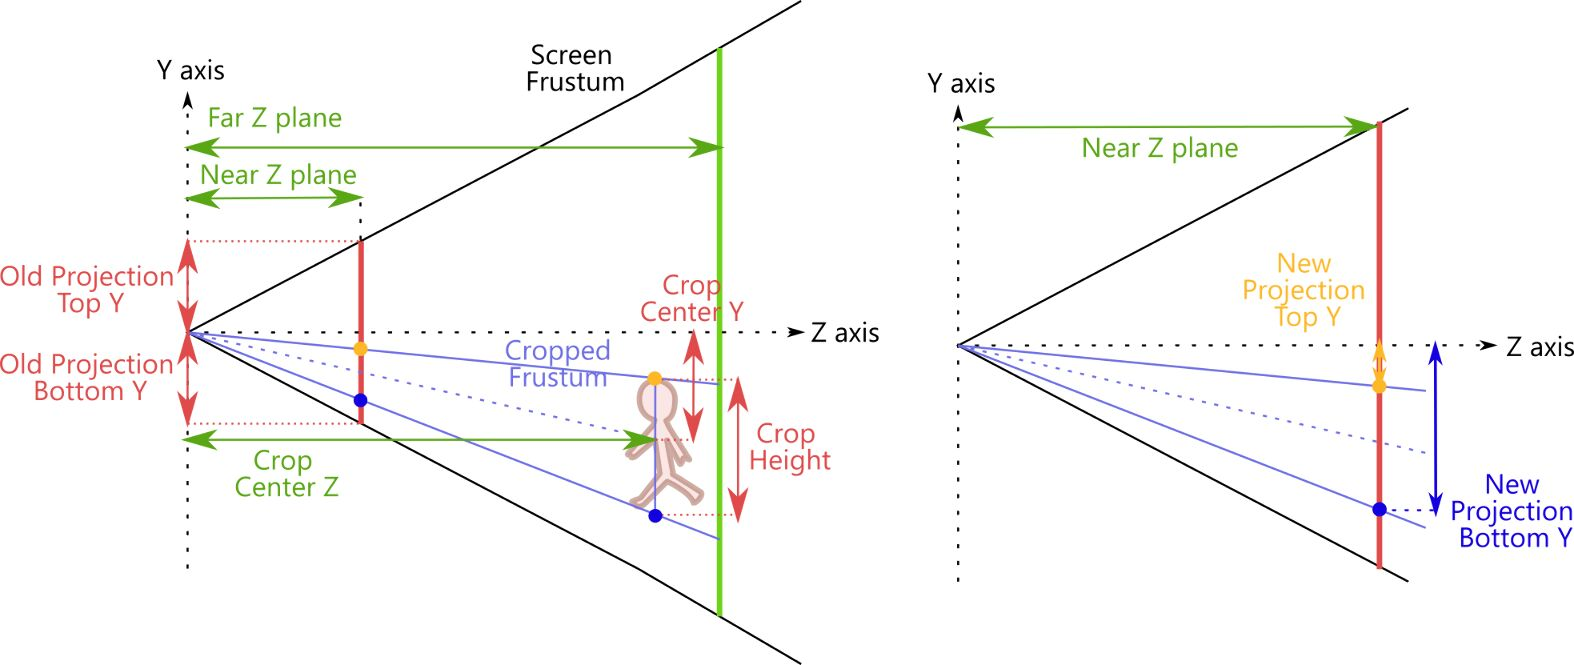
\includegraphics[width=\textwidth]{\imgfp/dynamic_crop/dynamic_crop}
%	%\setkeys{Gin}{draft}
%	\centering{\includegraphics[width=\textwidth]{test.eps}}
%	%\setkeys{Gin}{draft=false}
%	%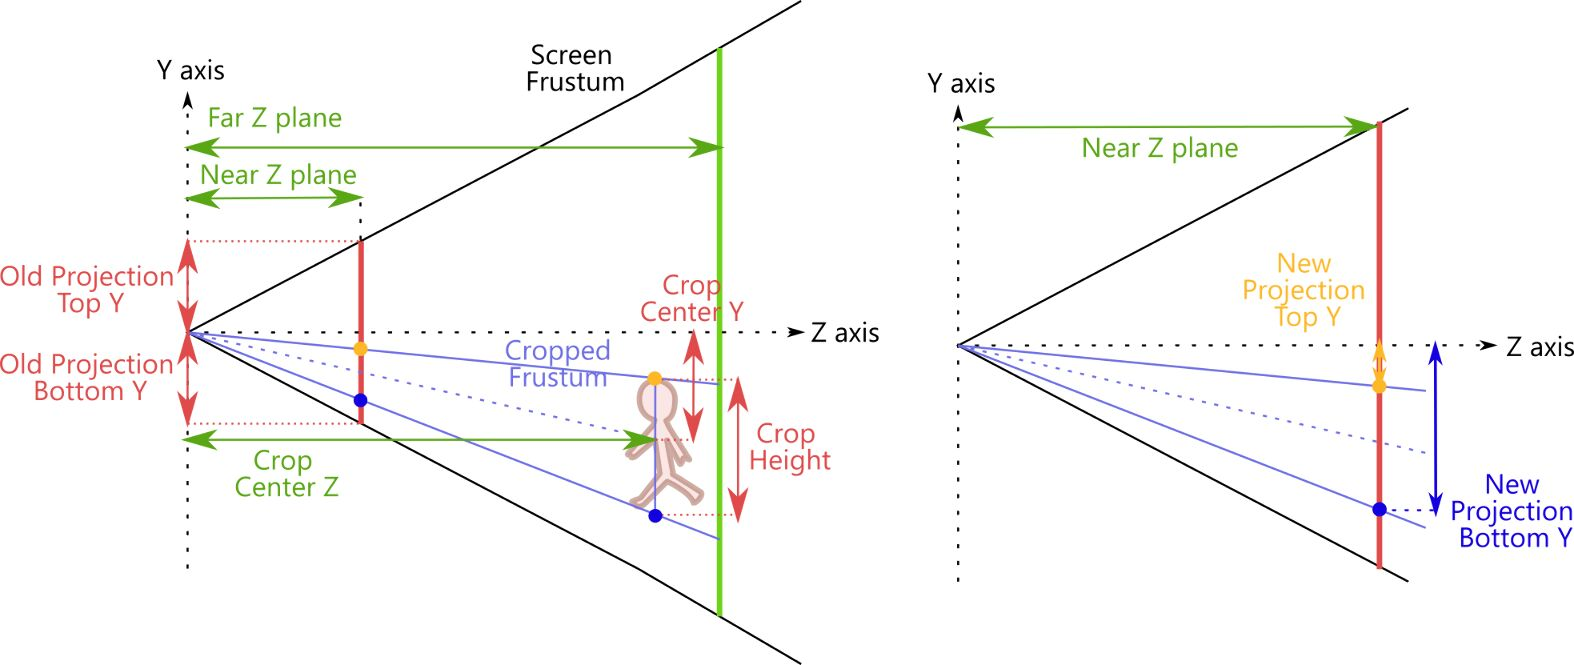
\includepdf[width=\textwidth]{\imgfp/dynamic_crop/dynamic_crop}
%	\caption{}
%\end{figure}

%\begin{figure}[h!]
%	\fboxrule=1pt
%	\centering
%	\begin{subfigure}[b]{0.495\textwidth}
%		\centering
%		\cfbox{gray}{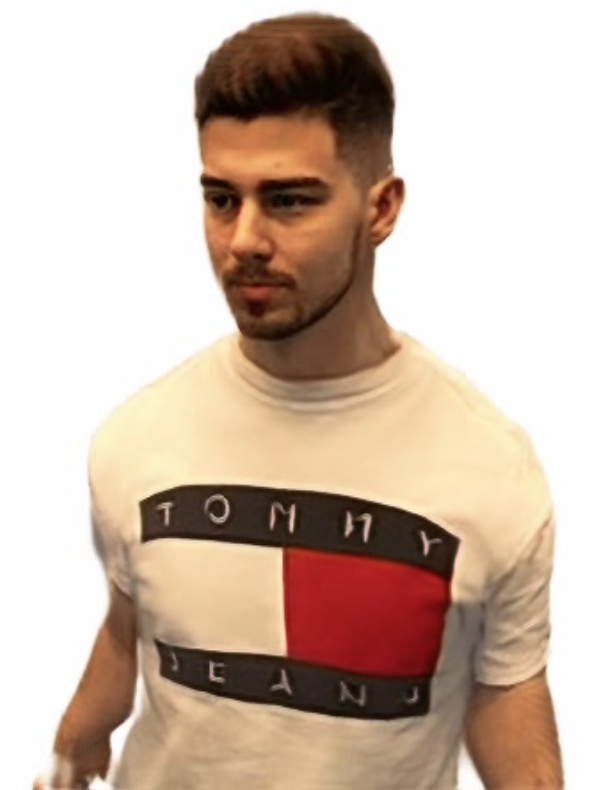
\includegraphics[height=10cm]{\imgfp/example_1}}
%		\caption{BNs collect statistics on FB frames}
%		\label{res:fig:example}
%	\end{subfigure}
%	\begin{subfigure}[b]{0.495\textwidth}
%		\centering
%		\cfbox{gray}{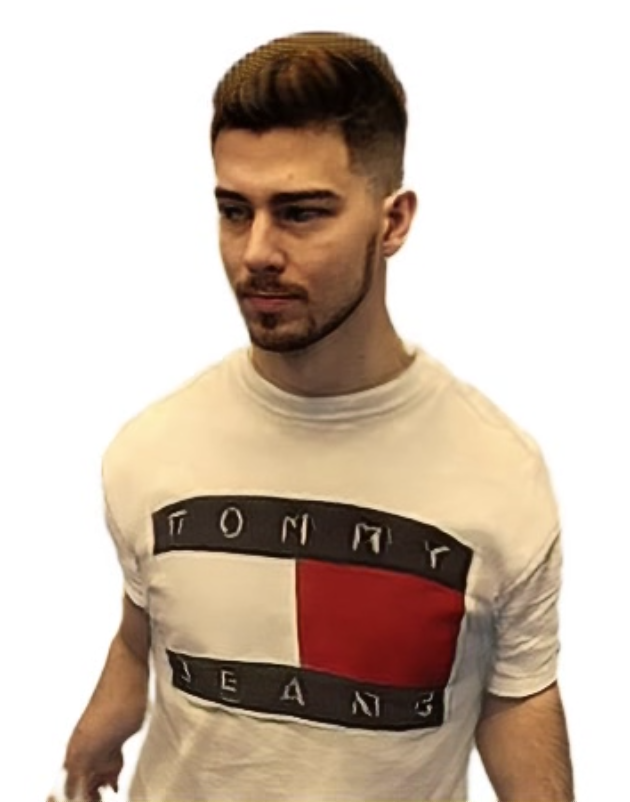
\includegraphics[height=10cm]{\imgfp/example_2}}
%		\caption{BNs collect statistics on zoomed frames}
%		\label{res:fig:example}
%	\end{subfigure}
%%	\centering
%%	\subcaptionbox{3a\label{fig3:a}}{\includegraphics[width=1.6in]{example-image-c}}\hspace{1em}%
%%	\subcaptionbox{3b\label{fig3:b}}{\includegraphics[width=1.6in]{example-image-c}}
%	\caption{Example}
%	\label{res:fig:example}
%\end{figure}

\section{Future work}\label{res:future}

The baseline model \cite{dnn:stylepeople21} is still state-of-the-art in its particular task -- rendering of a full-body avatar using information from a few monocular uncalibrated images, or a video sequence. However, as the original authors point out, it is an optimization-based approach that takes about half a day to converge, and may be impractical in a scenario where users can scan themselves and after a short time be able to use their avatars. The training time can be improved by doing further research on meta-learning, where both architecture and its initialization are sought, so that fine-tuning of it would converge to acceptable results after a very short optimization. On the other hand, a completely new algorithmic feed-forward solution could be proposed, so that a single inference would yield all the necessary data to generate realistic avatars.

Regarding this thesis project, the neural renderer's inference performance could be further improved. For example, we could employ already described approaches of knowledge distillation or neural architecture search, to find an architecture with fewer parameters, but similar visual quality. However, such research efforts are known to be notoriously big, in terms of experimentation and amount of computations. On the other hand, purely algorithmic tricks could be used. The approach of pipelining \cite{mobile:pipelining20} could be used, to split the network into independent stages, with the idea that as soon as a stage finishes computation on the given data, it could pass the data to the next stage, and at the same time accept new input for processing. In the context of the mobile execution, some parts can be executed on different computing units (GPU, DSP) and exchange the data using the shared memory. As was shown in the Section \ref{res:performance}, in the current implementation of the mobile inference there is some idleness of DSP between frames, caused by latency of rasterizing each new frame and sending it to the DNN. More efficient organization of calculations could be researched to minimize this idleness, potentially gaining about 10-15\% of performance. For example, CPU multithreading could be better utilized in the future, or batch inference of the DNN on mobile to improve throughput of data through the computing units.

Improving the quality of synthesized images is also a big field for research. Making small training procedure adjustments as was described in this thesis proved to be ineffective to solve all the current issues with overfitting and randomness. Thus, research on other architectures is yet again more preferable. This also requires to decide on generalization ability of the rendering architecture. On one hand, sticking to one-DNN-one-avatar approach, allows to obtain the full realism for the particular person. A lot of attention is brought to NeRF \cite{dnn:nerf20, dnn:phorhum22} based methods, from which very realistic images can be sampled from many novel views. On the other hand, it would be beneficial if a single DNN could be used to render many avatars, distinguishing them by neural textures. Thus we could place multiple different avatars in a single frame of AR, and generate images of all of them at once. 

Such scenario anticipates the dawn of true telepresence communication, given that mobile devices are already capable of doing real-time DNN inference. However, this would also require to overlook the cropping approach that was used in this thesis to get higher and stable visual quality. Imagine if we were to render two avatars separated by a considerable distance. By using a bounding box that includes both of them to do frustum cropping, both avatars will be quite small in the frame, once again bringing up the necessity for the DNN to be stable on far-views (as in Figure \ref{fig:far_screen_crop}) One way to extend cropping to a multi-avatar scenario, is to use the fact that in OpenGL we can rasterize to a part of an image. Thus, we could compute bounding boxes for each avatar separately, then to distribute the input frame between avatars rasterizations, proportional to used image area in AR (See Figure \ref{fig:multiavatar}). An additional advantage is that we do not need to worry about avatars overlapping, because they will be rasterized one by one, without affecting each other. The time of rasterizing $N$ avatars is still extremely smaller than a DNN inference time. The proportion of areas on the input frame can also be dynamically adjusted to yield better images for nearby avatars, and decreasing quality of far-away ones.

Lastly, the issue of stability in rendering unseen body parts has to be tackled. In this thesis we used a handcrafted solution to replace the corresponding texture parts with content that was seen by the neural renderer. However, we believe, that a more general algorithmic approach could be used, e.g. by inpainting the neural texture with logical content, or by feeding the renderer during training with images that show the missed body parts, even though the training sequence does not contain them. These could be images of other people, augmented to match the hair or clothes colors. Or these could be synthesized from some other model that saw these body parts.
%\begin{enumerate}
%	\item To use shared memory between GPU and DSP, to eliminate sending of OpenGL rasterized images between GPU and DSP
%	\item To use bufferization of data to infer DNN in batches (possibly better DSP usage ratio)
%	\item To research on training a single renderer for multiple people, and adjusting mobile inference to fit multiple people simultaneously. We can render multiple avatars in different corners of an input rasterization, regardless of distance in camera space. Then after getting an output image, we can tear apart this image and place corresponding avatars in different places of the AR space.
%	\item To research on completely different neural rendering architectures, since the small adjustments of the current baseline yield little to no benefit
%	\item To find an algorithmic way of solving the issue of unseen body parts during training
%	\item To research on other regularizing techniques to prevent overfitting, without harming high-frequency details learning 
%\end{enumerate}